%!TEX root = ../Final_Assignment_SP_ML4IM_2023.tex
\chapter{Results}
\label{ch:results}

% ausführlich
% alle

This chapter presents the results of the project. This is done by visualising and comparing the results of the different data pre-processing approaches.

% RGB
First af all the results of the default RGB training are presented. The default RGB training was done using the raw RGB data without any preprocessing. The results of this training are shown in Table~\ref{fig:results_rgb}.

% results of rgb
The important values to look at are the precision and recall of the model epochs. The precision and recall values should be as high as possible. The precision value shows the accuracy of the detected objects and the recall value shows how many of the actual values were correctly predicted. Normally the two values get better as more epochs are processed \citep{ultralyticsYOLOPerformance}. But in the figure \ref{fig:results_rgb} the precision gets lower with each new epoch, except for one spike, and the recall stays quite low with one low point.
The box\_loss is also an interesting value to look at. It shows the loss of the bounding boxes. The lower the value, the better the bounding boxes are predicted. The box\_loss gets lower with each epoch, which at first sight is a good sign. But the box loss of the validation varies a lot. So this model is quite bad at detecting the insects in the RGB data.

\begin{figure}[htbp] 
    \centering
    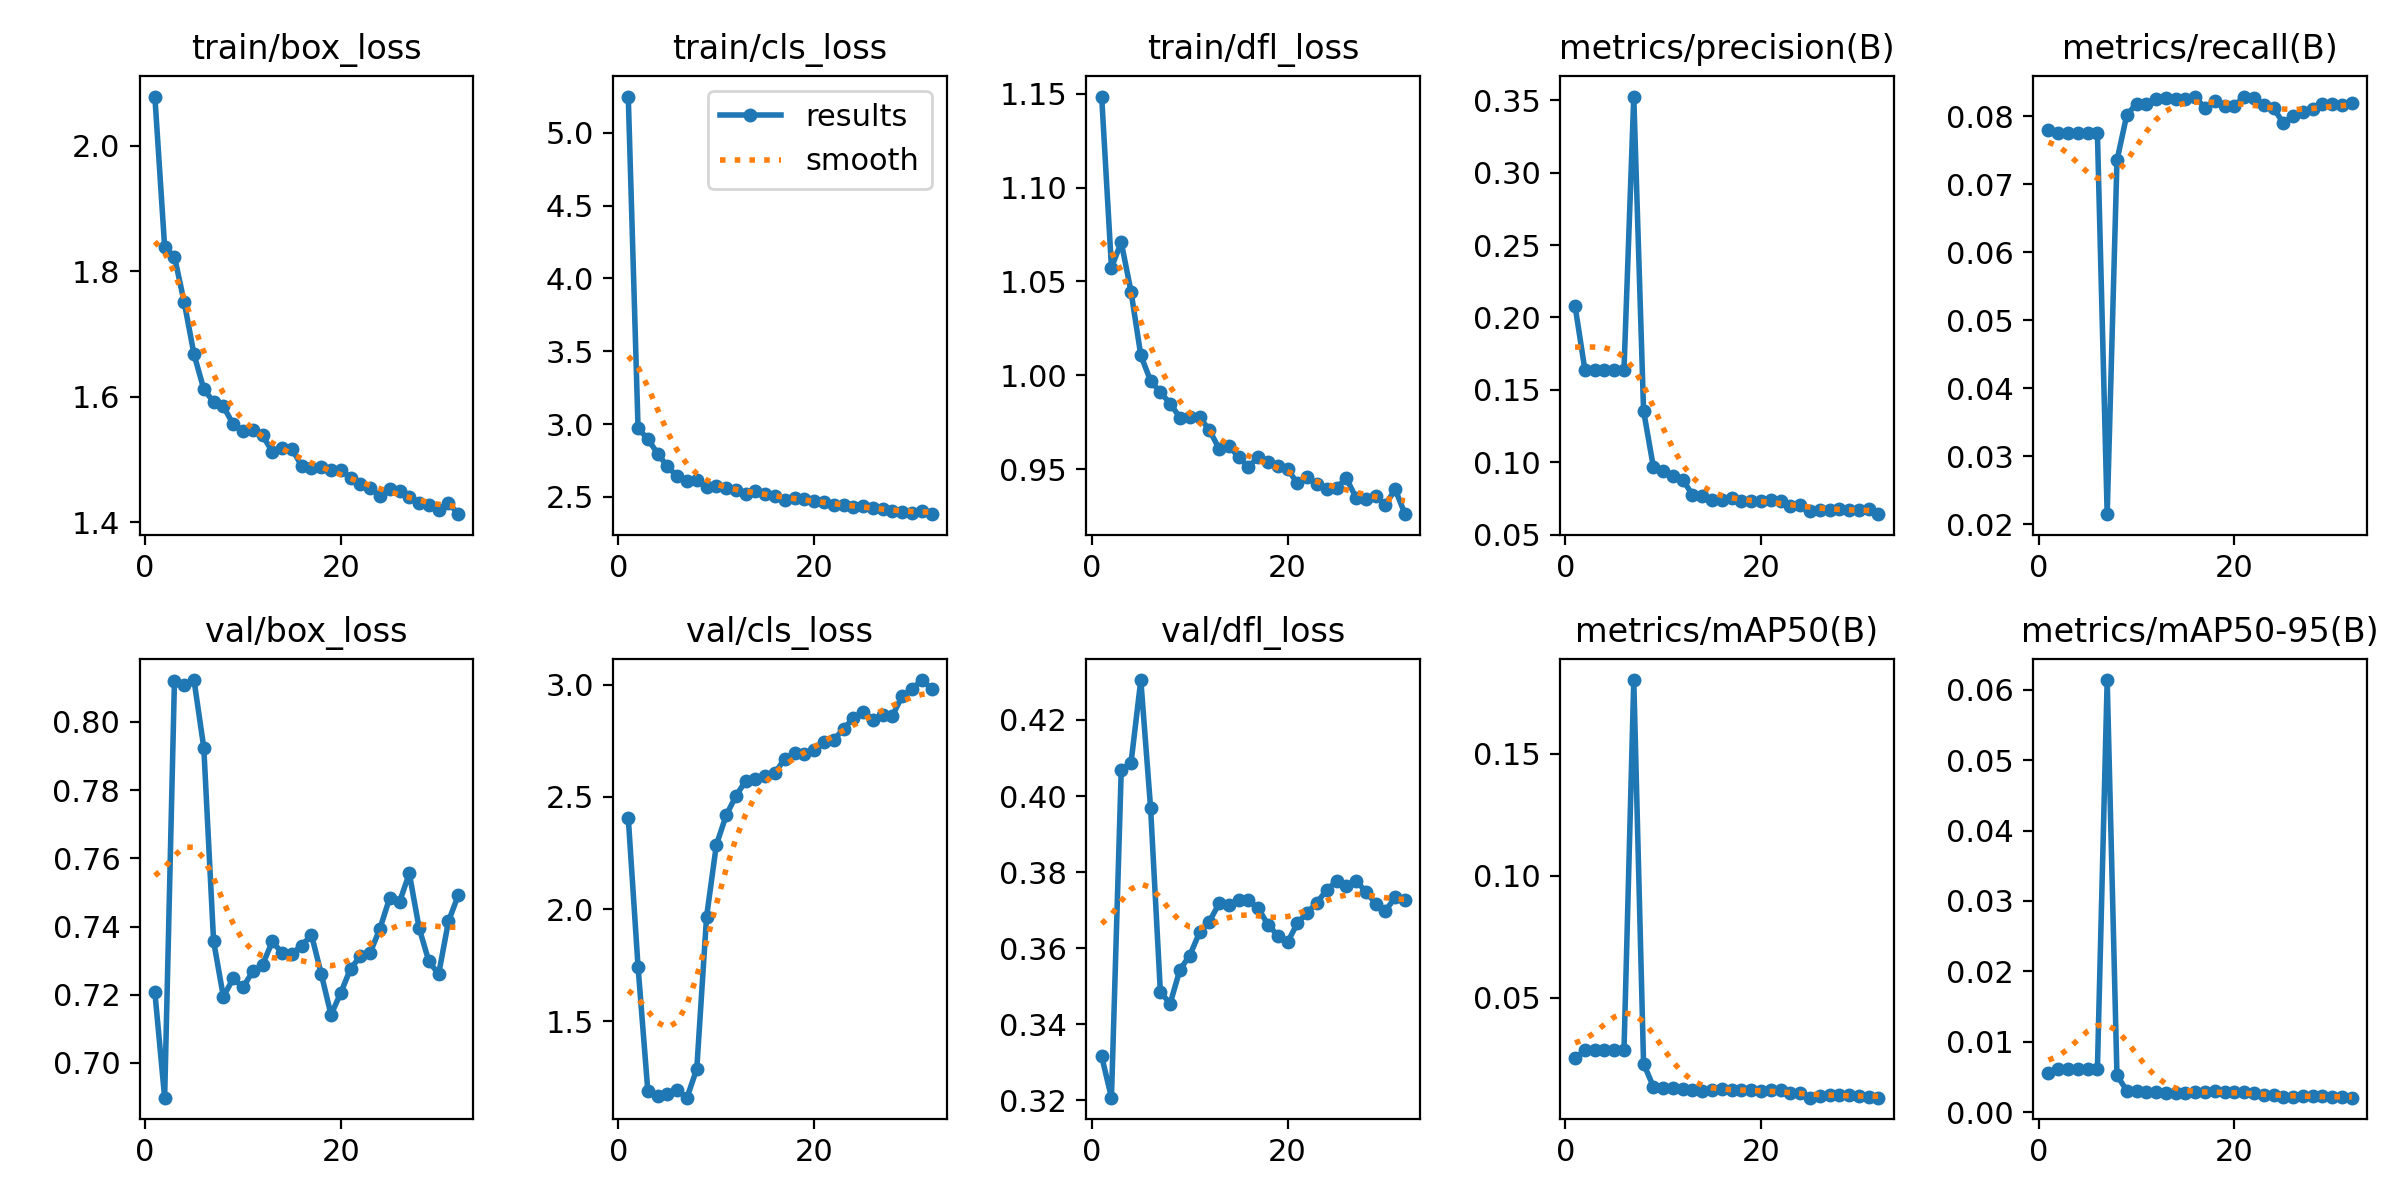
\includegraphics[width=0.8\textwidth]{images/results/rgb_results.png}
    \caption{Results of the model training with RGB data}
    \label{fig:results_rgb}
\end{figure}

% background subtraction

The background subtraction method was then used on the rgb data. The results of this training are shown in Table~\ref{fig:results_bgsub}.

\begin{figure}[htbp] 
    \centering
    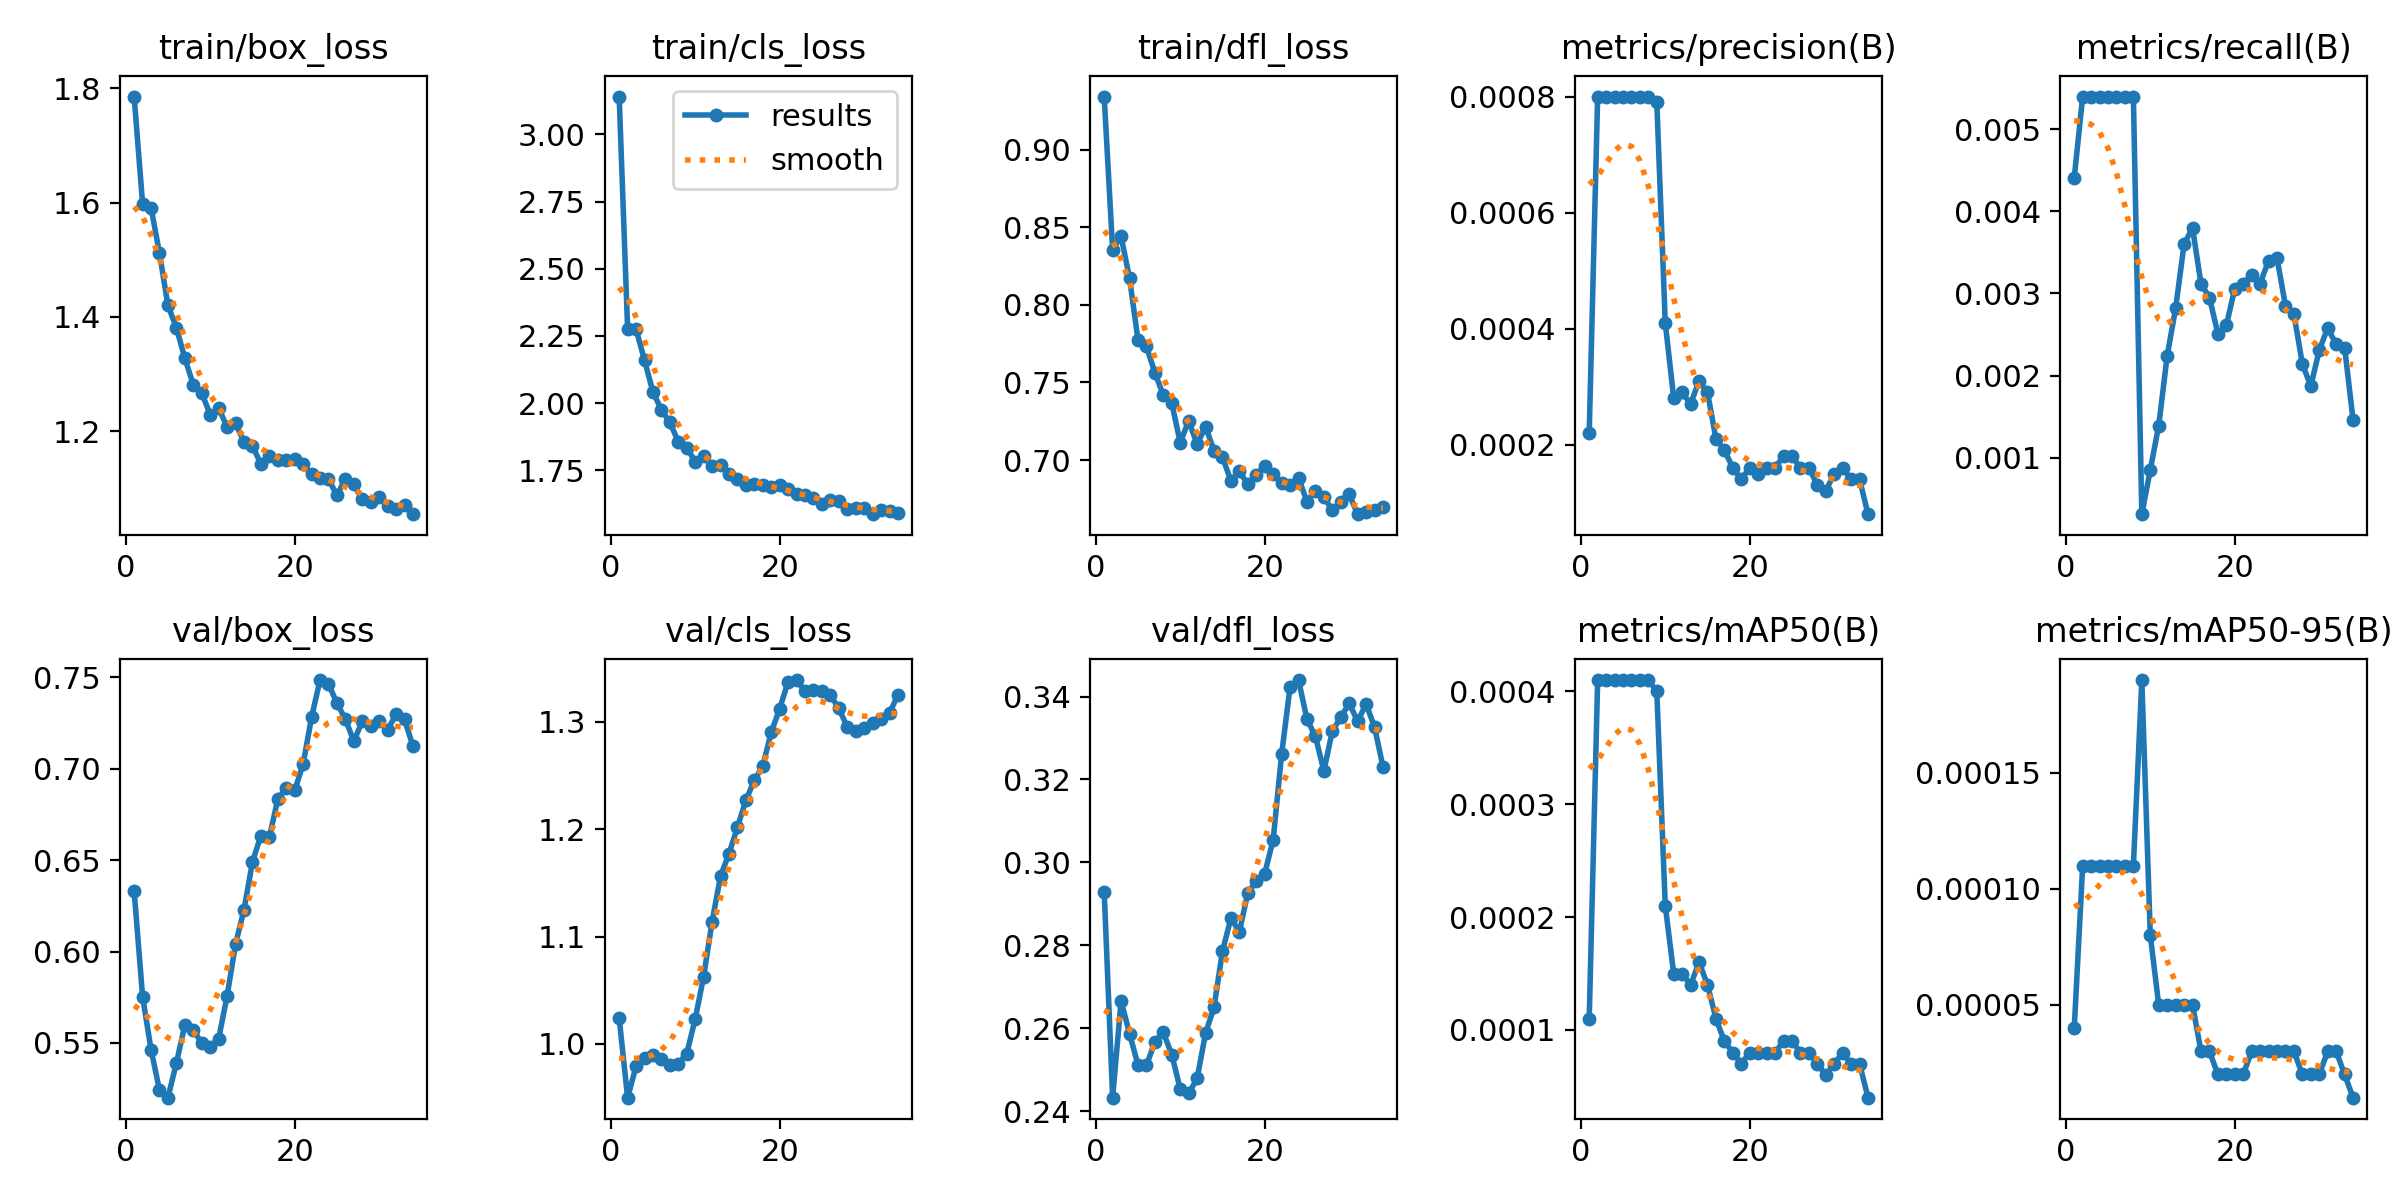
\includegraphics[width=0.8\textwidth]{images/results/bgsub_results.png}
    \caption{Results of the model training with background subtraction}
    \label{fig:results_bgsub}
\end{figure}

% results of background subtraction
The background subtraction model has much lower precision and recall than the RGB model. In the final epochs it goes down to less than 0.0002, but the box\_loss looks normal. All in all, the results of the background subtraction model are not good and should normally be better than the RGB model.

% background subtraction + time offset 1

The background subtraction method was then combined with the time offset method with an offset of 1. The results of this training are shown in Table~\ref{fig:results_bgsub_timeoffset1}.

\begin{figure}[htbp] 
    \centering
    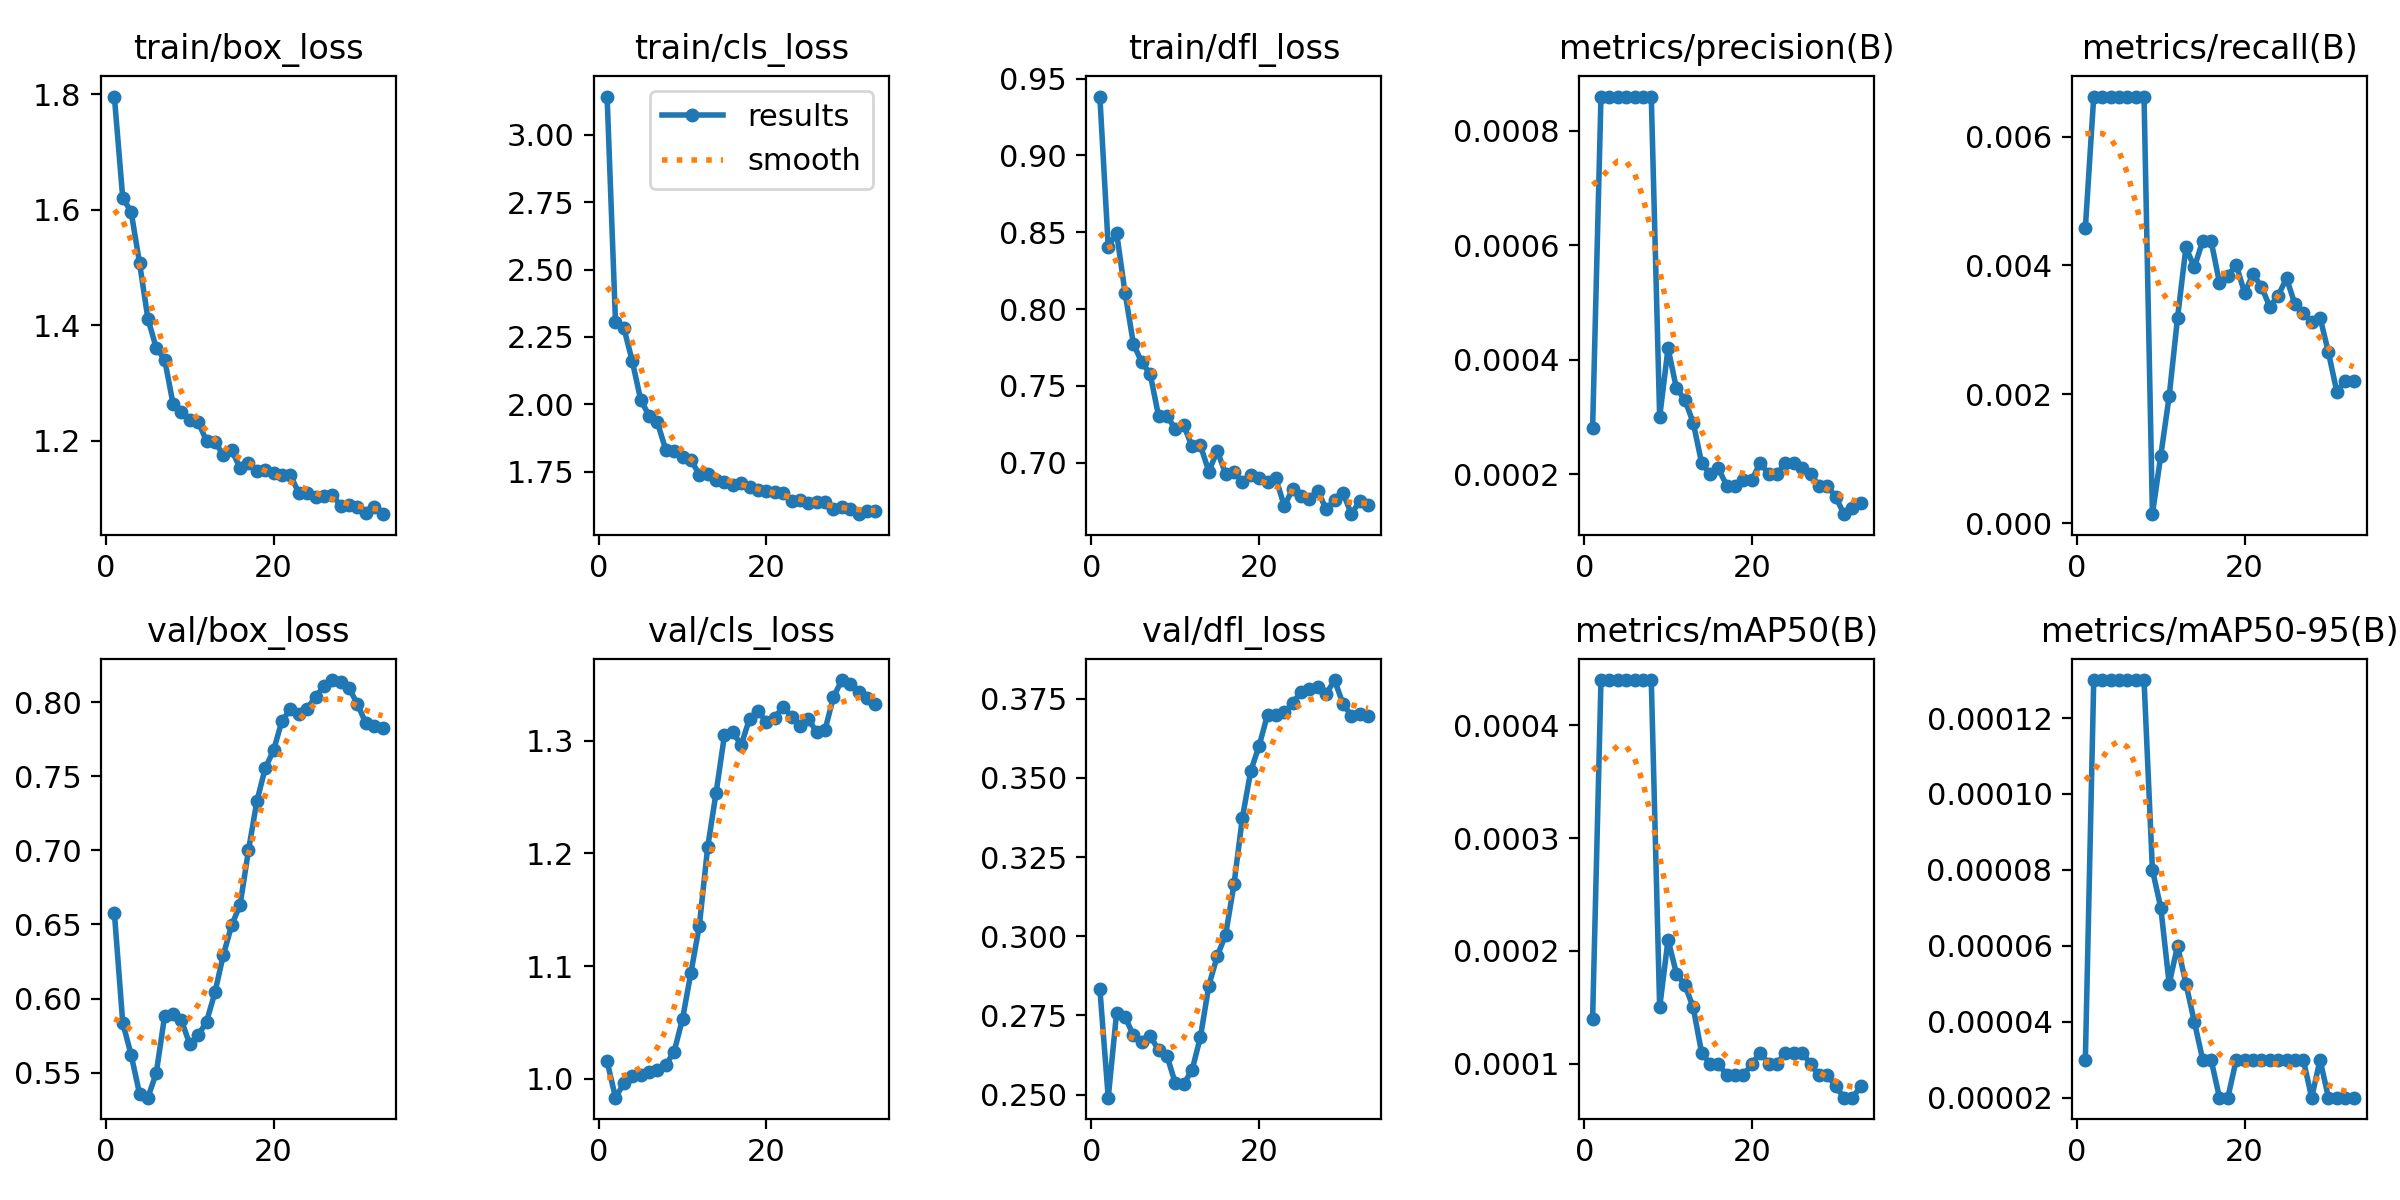
\includegraphics[width=0.8\textwidth]{images/results/bgsub_timeoffset1_results.png}
    \caption{Results of the model training with background subtraction and time offset 1}
    \label{fig:results_bgsub_timeoffset1}
\end{figure}

% results of background subtraction + time offset 1
Because the frames in the video data were simply combined with an extra frame to visualise movement in the images, the results of the background subtraction + time offset 1 model are similar to the background subtraction model, with almost the same results. So the time offset had no effect on the model.

% HSV
The next results are from the training with the HSV data. The HSV data was created by converting the RGB data to the HSV color space. The results of this training are shown in Table~\ref{fig:results_hsv}.

\begin{figure}[htbp] 
    \centering
    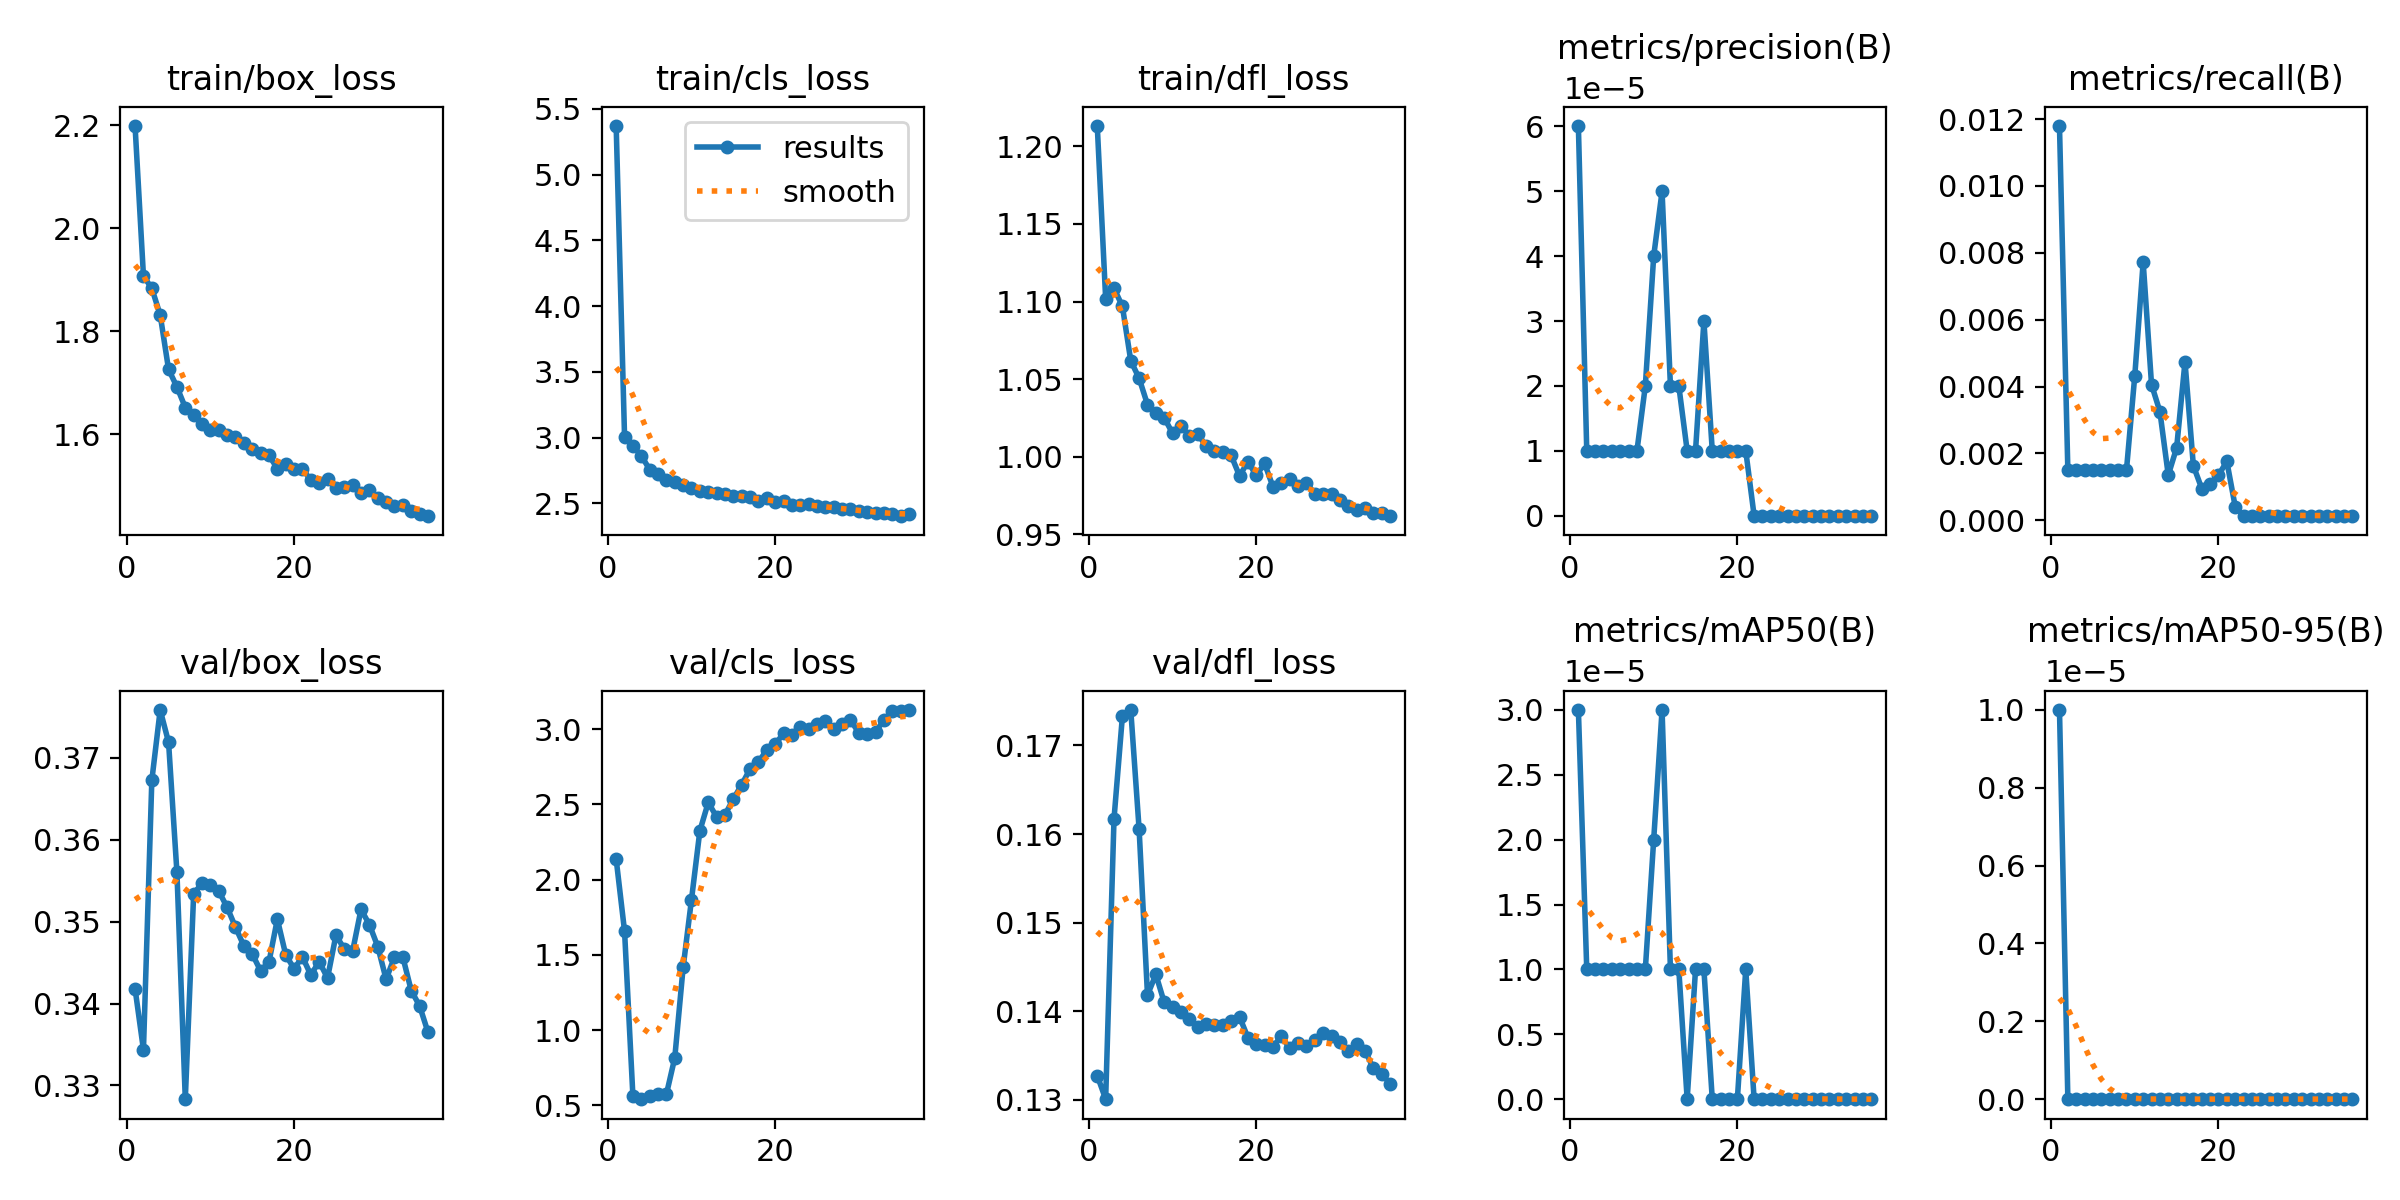
\includegraphics[width=0.8\textwidth]{images/results/hsv_results.png}
    \caption{Results of the model training with HSV data}
    \label{fig:results_hsv}
\end{figure}

% results of hsv
The precision and recall of the HSV training are very low. They do not increase steadily as they should, and in the later epochs they are even close to zero. This is a really abnormal progression. The box loss actually goes down steadily, which is a good sign. These results show that the model is not able to detect the insects in the HSV data.

% HSV + background subtraction
The HSV data was then combined with the background subtraction method. The results of this training are shown in Table~\ref{fig:results_hsv_bgsub}.

\begin{figure}[htbp] 
    \centering
    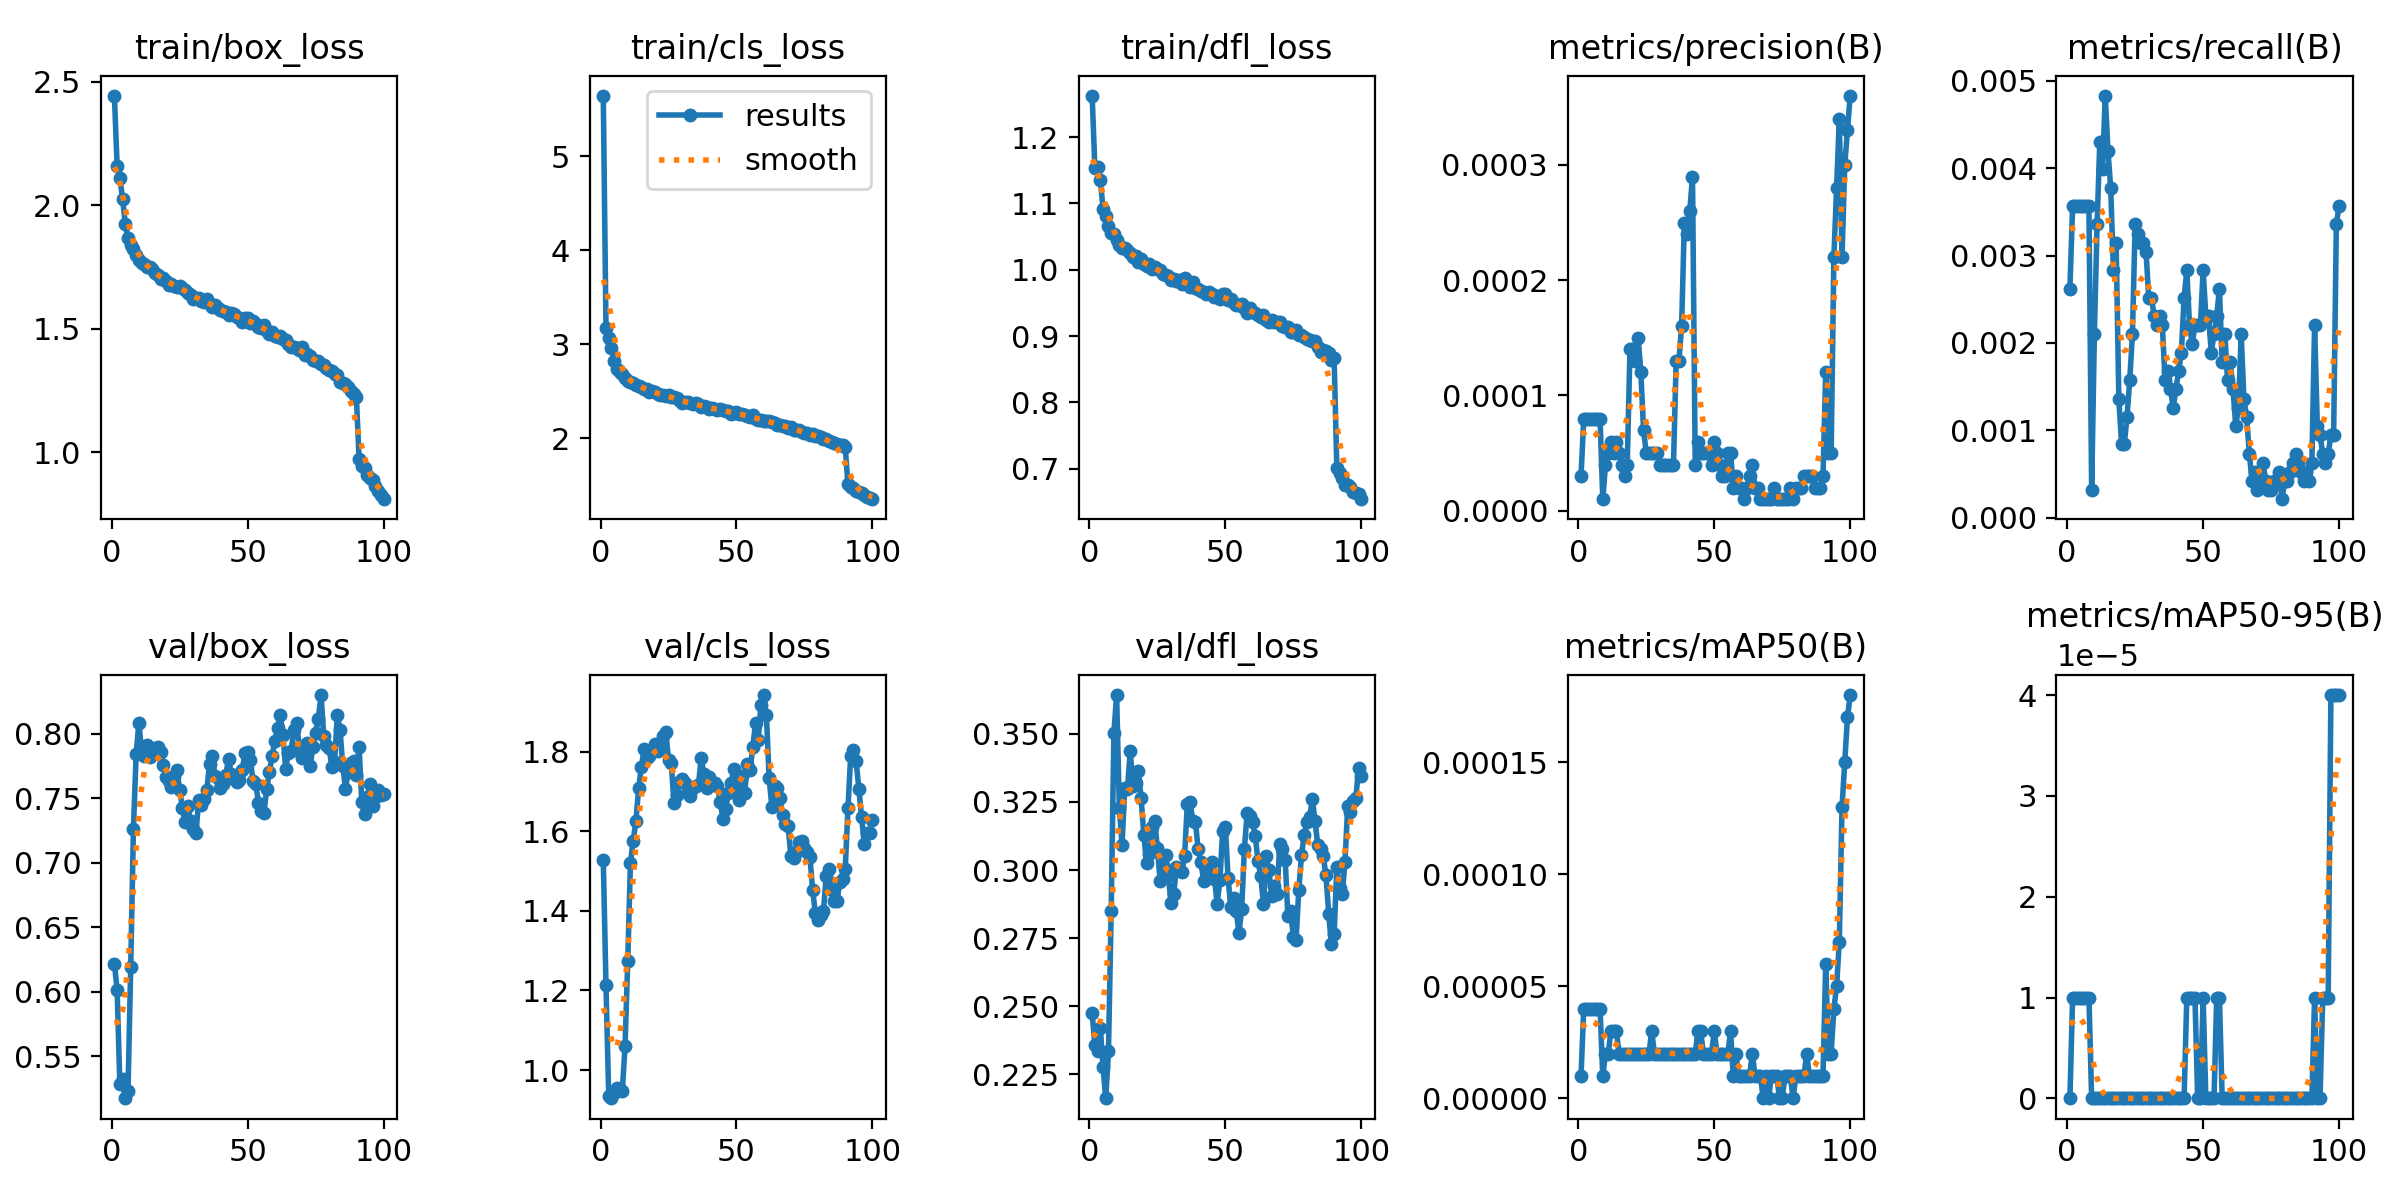
\includegraphics[width=0.8\textwidth]{images/results/hsv_bgsub_results.png}
    \caption{Results of the model training with HSV data and background subtraction}
    \label{fig:results_hsv_bgsub}
\end{figure}

% results of hsv + background subtraction
The results of the model trained with the HSV data and background subtraction are based on the same data as the HSV model. With the background subtraction added, the model should perform better than the original HSV model. First, the precision and recall values are higher than the original HSV model, but still close to zero. As the precision and recall values do not look normal, the model is not able to detect the insects in the HSV data with the background subtraction.

Further analysis is not necessary due to the poor results of the models. Other findings of the models do not provide any more valuable information. In the next chapter these results are discussed and possible reasons for the poor results are given.
